
\section{Function Oriented}

Object-oriented design is the process of planning a system of interacting objects for the purpose of solving a software problem. It is one approach to software design. An object contains encapsulated data and procedures grouped together to represent an entity. The 'object interface' defines how the object can be interacted with. An object-oriented program is described by the interaction of these objects. Object-oriented design is the discipline of defining the objects and their interactions to solve a problem that was identified and documented during object-oriented analysis.

\iffalse
 basic requirement of this app is that the user must be having ANDROID
Operating System in his phone or tablet. The minimum version of Androids Operating
System must be ICECREAM SANDWICH. All the versions of Android OS above
IcecreamSandwich( i.e. Jellybean, Kitkat, Lollipop,Marshmallows) will support this
app. A user needs Monitary app installed in device .


\noindent As shown in the Figure \ref{fig:1}, .\\Brief introduction showing the features available in the application.

\begin{figure}[ht]
\centering
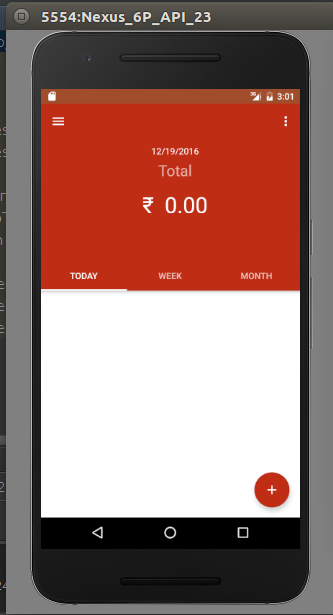
\includegraphics[scale=0.5]{images/s1.png}
\caption{Screen 1}
\label{fig:1}
\end{figure}

\noindent This are the options the navigation drawer the app will contain. These will contain the screens the user can navigate too that can be seen in Figure \ref{fig:2}. \\

\begin{figure}[ht]
	\centering
	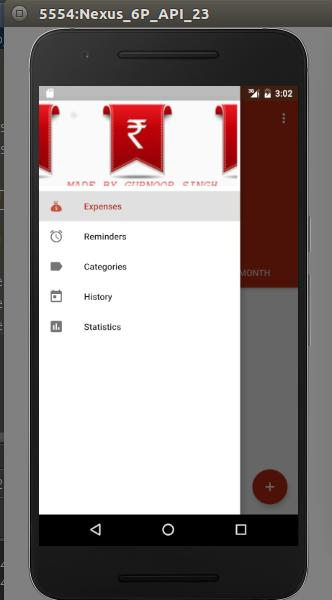
\includegraphics[scale=0.49]{images/s2.png}
	\caption{Screen 2}
	\label{fig:2}
\end{figure}

\noindent  Statistics will be able to change according to the dates selected. Default values will be the current week. User Will be able to see diagrams according to Quantity and
days, Quantity and categories and others.as seen in the Figure \ref{fig:3}.\\

\begin{figure}[ht]
\centering
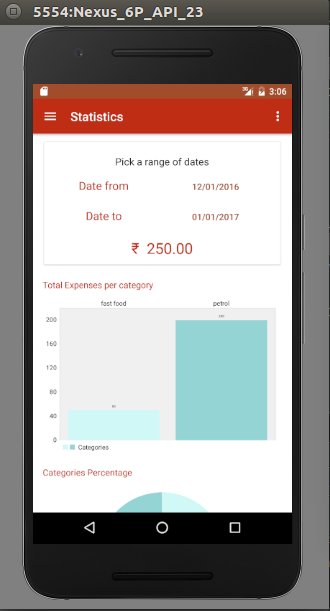
\includegraphics[scale=0.5]{images/s3.png}
\caption{Screen 3}
\label{fig:3}
\end{figure}

\noindent Reminder view will contain details from the reminder created and the user can edit
the reminder values. in Figure \ref{fig:4}. \\

\begin{figure}[ht]
\centering
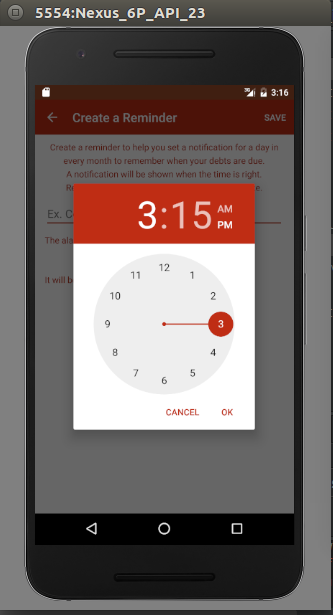
\includegraphics[scale=0.38]{images/s4.png}
\caption{Screen 4}
\label{fig:4}
\end{figure}

\noindent Reminder screen will show the current saved Reminder and if they are active or not.
To activate one it will have a switch next to the name so it can be activated in any
moment. The user will be able to erase and add from this view as seen in the Figure \ref{fig:5}. It's named as output.dxf. We can open that file in LibreCAD directly from the command-line.\\


\begin{figure}[ht]
\centering
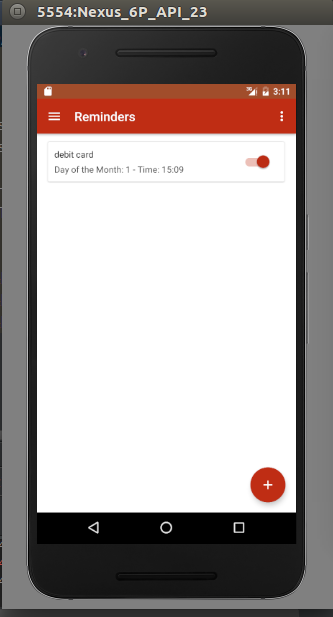
\includegraphics[scale=0.5]{images/s6.png}
\caption{Screen 5}
\label{fig:5}
\end{figure}

\noindent Expenses View is the main screen that will be showed. The user will be able to add expenses and see a total amount in Today, Week and Month. as shown in Figure \ref{fig:6}. 

\begin{figure}[ht]
\centering
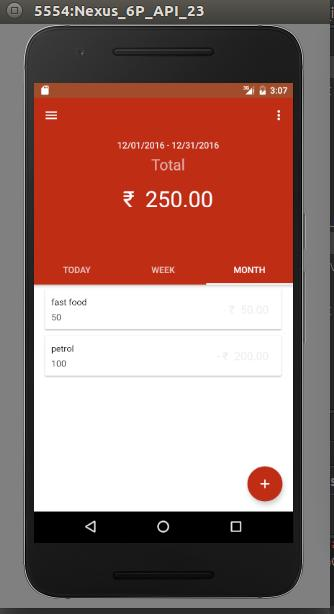
\includegraphics[scale=0.38]{images/s61.png}
\caption{Screen 6}
\label{fig:6}
\end{figure}

\noindent This activity will provide necessary help to the user. One can also mail the maker
(GURNOOR SINGH) for further queries as shown in Figure \ref{fig:7}. 

\begin{figure}[ht]
\centering
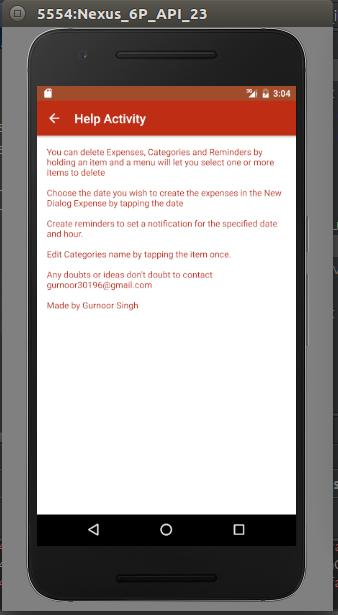
\includegraphics[scale=0.38]{images/s7.png}
\caption{Screen 7}
\label{fig:7}
\end{figure}
\noindent User will be able to add and delete categories from the Categories View \ref{fig:8}. 

\begin{figure}[ht]
\centering
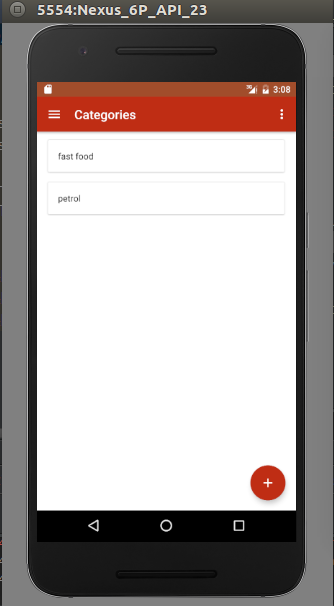
\includegraphics[scale=0.38]{images/s8.png}
\caption{Screen 8}
\label{fig:8}
\end{figure}
\fi

\section{Detail Design}